\chapter{Componentes, memória e tipos de dados}
\label{cap:memoria}

\begin{objetivos}
Ao final deste capítulo você deve ser capaz de:
\begin{itemize}
  \item descrever a função do microprocessador e dos blocos de memória;
  \item classificar memórias quanto ao acesso, à volatilidade e à forma de armazenamento;
  \item calcular a quantidade de bits de endereçamento de uma memória;
  \item reconhecer os tipos de dados elementares da norma e suas faixas de valor;
  \item aplicar o princípio da forte tipação e utilizar funções de conversão explícita de tipos;
  \item representar números negativos em complemento de dois;
  \item interpretar os campos dos formatos simples e duplo da IEEE-754;
  \item localizar as seis áreas do mapa de memória de um CLP.
\end{itemize}
\end{objetivos}

\section{O microprocessador e a memória}

O microprocessador é a inteligência do controlador: coleta os dados dos cartões de entrada, processa
segundo o programa do usuário, armazenado em memória, e envia o resultado aos cartões de saída.
A memória é o que dá sentido a esse processo --- guarda as instruções e os dados necessários para
executá-las.

\index{memória!de CLP}\index{microprocessador}

\section{Classificação das memórias}

Uma mesma memória pode ser descrita por quatro critérios independentes
(Tabela~\ref{tab:classificacao-memoria}).

\begin{table}[H]
  \centering
  \caption{Critérios de classificação de memórias.}
  \label{tab:classificacao-memoria}
  \begin{tabular}{p{3.0cm} p{5.0cm} p{6.6cm}}
    \toprule
    Critério & Categorias & Exemplo e consequência \\
    \midrule
    Acesso
      & Sequencial: chega à posição passando pelas intermediárias. Aleatório ou direto: chega
diretamente à posição endereçada
      & Fita magnética (sequencial) e semicondutores (direto). O \emph{tempo de acesso} é o
intervalo entre a entrada do endereço e a informação disponível na saída \\
    Volatilidade
      & Volátil: perde o conteúdo sem alimentação. Não volátil: mantém o conteúdo
      & RAM é volátil; ROM, PROM e EPROM são não voláteis \\
    Escrita e leitura
      & Escrita e leitura, ou somente leitura
      & RAM permite ambas; ROM permite apenas leitura \\
    Forma de armazenamento
      & Estática: o dado permanece indefinidamente. Dinâmica: exige reinserção periódica
      & Estática em flip-flop; dinâmica em capacitor \\
    \bottomrule
  \end{tabular}
\end{table}

\section{Tecnologias de memória}

\begin{table}[H]
  \centering
  \caption{Tecnologias de memória presentes em controladores.}
  \label{tab:tecnologias-memoria}
  \begin{tabular}{p{2.6cm} p{5.4cm} p{6.6cm}}
    \toprule
    Tecnologia & O que é & Característica de uso \\
    \midrule
    ROM de máscara
      & Somente leitura, gravada pelo fabricante
      & Não volátil, não permite apagamento \\
    PROM
      & Programável uma única vez, gravada pelo usuário
      & Não volátil, não permite apagamento \\
    EPROM
      & Programável e apagável por exposição a ultravioleta
      & Não volátil; exige programador dedicado, o que encarece a manutenção \\
    EEPROM
      & Apagável e regravável eletricamente
      & Não volátil; escrita e leitura bem mais lentas que a RAM \\
    EAROM
      & Regravável eletricamente
      & Não volátil e reprogramável, porém lenta \\
    RAM estática
      & Acesso aleatório, com armazenamento em flip-flop
      & Volátil, rápida, ocupa mais espaço e custa mais \\
    RAM dinâmica
      & Acesso aleatório, com armazenamento em capacitor
      & Volátil, mais lenta, ocupa menos espaço e custa menos \\
    NOVRAM
      & RAM mantida por acumulador ou bateria
      & Mantém o conteúdo por meses sem alimentação, com velocidade de RAM e custo elevado \\
    FLASH
      & Substituta da ROM e da EPROM
      & Não volátil, alta confiabilidade, menor consumo e gravação elétrica \\
    \bottomrule
  \end{tabular}
\end{table}

\section{Endereçamento, barramentos e cálculo de memória}

Uma memória eletrônica tem três barramentos: \textbf{endereços}, \textbf{dados} e
\textbf{controle}. O barramento de dados é bidirecional --- é o que caracteriza uma memória de
leitura e escrita. A capacidade é indicada pela notação $N \times m$, em que $N$ é o número de
localidades e $m$ o número de bits por localidade: $256\times8$, $1\text{K}\times16$,
$128\text{M}\times32$.

Nessa notação, $\text{K} = 2^{10} = 1.024$ e $\text{M} = 2^{20} = 1.048.576$. A relação entre
capacidade e bits de endereçamento é:

\begin{equation}
  N_{\text{total}} = m \times 2^{\,n_{\text{end}}}
  \qquad\Longleftrightarrow\qquad
  n_{\text{end}} = \log_2\!\left(\frac{N_{\text{total}}}{m}\right)
  \label{eq:calculo-memoria}
\end{equation}

\paragraph{Exemplo 1.} Um dispositivo com $393.216$ bits no total e palavras de $12$ bits:

$$
2^{x} = \frac{393.216}{12} = 32.768 \quad\Longrightarrow\quad
x = \log_2 32.768 = 15 \text{ bits de endereçamento}
$$

\paragraph{Exemplo 2.} Uma memória $128\text{M} \times 32$: como $128\text{M}$ é
$128 \times 2^{20}$, o total é $128 \times 2^{20} \times 32 = 4.294.967.296$ bits e o número de
palavras é $134.217.728$, o que exige $27$ bits de endereçamento.

\begin{atencao}
Um erro clássico é confundir o número de \emph{palavras} com o número de \emph{bits}. Uma memória
$128\text{M}\times32$ tem $128$ milhões de palavras e $4$ bilhões de bits. A faixa de endereços
--- e portanto os bits de endereçamento --- depende do número de palavras, não do total de bits.
\end{atencao}

\section{Tipos de dados da norma}

Os tipos de dados especificam o valor que cada variável pode assumir e como esse valor é organizado
na memória. Os tipos elementares definidos pela IEC 61131-3 são apresentados na
Tabela~\ref{tab:tipos-dados}.

\begin{table}[H]
  \centering
  \caption{Tipos de dados elementares e faixas de valor.}
  \label{tab:tipos-dados}
  \begin{tabular}{l p{4.6cm} r p{4.4cm}}
    \toprule
    Tipo & Significado & Bits & Faixa de valor \\
    \midrule
    BOOL   & Booleano: falso ou verdadeiro, 0 ou 1 & 1  & 0 ou 1 \\
    SINT   & \emph{Short integer}, inteiro curto com sinal & 8  & $-128$ a $127$ \\
    INT    & \emph{Integer}, inteiro com sinal & 16 & $-32.768$ a $32.767$ \\
    DINT   & \emph{Double integer}, inteiro duplo com sinal & 32 & $-2.147.483.648$ a $2.147.483.647$ \\
    USINT, BYTE & Inteiro curto sem sinal & 8 & $0$ a $255$ \\
    UINT, WORD  & Inteiro sem sinal & 16 & $0$ a $65.535$ \\
    UDINT, DWORD & Inteiro duplo sem sinal & 32 & $0$ a $4.294.967.295$ \\
    REAL   & Real em ponto flutuante, precisão simples & 32 & $\pm1,18\times10^{-38}$ a $\pm3,40\times10^{38}$ (7 dígitos) \\
    LREAL  & Real em ponto flutuante, precisão dupla & 64 & $\pm2,23\times10^{-308}$ a $\pm1,80\times10^{308}$ (15 dígitos) \\
    TIME   & Duração, em milissegundos & 32 & $0$ a $4.294.967.295$\,ms \\
    \bottomrule
  \end{tabular}
\end{table}

Note a diferença entre \emph{com sinal} e \emph{sem sinal}: o tipo com sinal usa o bit mais
significativo para representar o sinal, e por isso tem metade da faixa positiva, ganhando a mesma
faixa em valores negativos.

\index{tipos de dados}\index{forte tipação}

\subsection{Declaração de variáveis e o princípio da forte tipação}

Na norma IEC 61131-3, todo dado manipulado pelo programa deve pertencer a uma variável expressamente
declarada com seu respectivo tipo de dado. O modelo adota o princípio da \textbf{forte tipação}
(\emph{strong typing}). Diferentemente de linguagens de script ou de uso geral que permitem coerção
implícita (\emph{implicit type casting}), os compiladores de CLP exigem correspondência estrita de
tipos em qualquer operação ou atribuição.

Em sistemas industriais, a forte tipação não é uma restrição burocrática, mas uma exigência crítica
de \textbf{segurança operacional}:
\begin{itemize}
  \item impede que truncamentos automáticos descartem frações decimais em malhas de controle;
  \item evita estouros de capacidade (\emph{overflow}) silenciosos que poderiam inverter o sinal de
        um comando ou zerar contadores de segurança;
  \item impede que grandezas físicas incompatíveis (como somar uma contagem de peças em \texttt{INT}
        com um intervalo de tempo em \texttt{TIME}) sejam combinadas por engano do programador.
\end{itemize}

A declaração formal de variáveis na IEC 61131-3 ocorre em blocos delimitados por \texttt{VAR} e
\texttt{END\_VAR}, conforme ilustrado na Listagem~\ref{lst:declaracao-tipos}.

\begin{lstlisting}[language=, caption={Declaração de variáveis com tipos distintos na IEC 61131-3.}, label={lst:declaracao-tipos}]
VAR
    bBombaLigada      : BOOL;   // Estado logico do atuador (TRUE ou FALSE)
    iLeituraBruta     : INT;    // Contagem de 16 bits do cartao analogico (-32768 a 32767)
    diTotalizador     : DINT;   // Contador acumulado de ciclos de producao (32 bits)
    rPressaoBar       : REAL;   // Pressao calculada do processo em bar (IEEE-754, 32 bits)
    tTempoMistura     : TIME;   // Duracao da etapa de dosagem (ex.: T#30s)
END_VAR
\end{lstlisting}

\subsection{Incompatibilidade direta entre tipos: o que não compila}

O conceito fundamental que todo estudante e projetista de automação deve dominar é: \textbf{não é
possível operar, comparar ou atribuir variáveis de tipos diferentes diretamente}. Se o código tentar
misturar variáveis de tipos distintos sem conversão explícita, o ambiente de desenvolvimento
acusará \textbf{erro fatal de compilação} e se recusará a gerar o código executável para a CPU do
controlador.

A Listagem~\ref{lst:erros-tipos} exemplifica quatro erros clássicos cometidos por iniciantes que
são prontamente barrados pelo compilador.

\begin{lstlisting}[language=, caption={Operações inválidas rejeitadas pelo compilador por incompatibilidade de tipo.}, label={lst:erros-tipos}]
// ERRO 1: Atribuicao direta de REAL para INT
iLeituraBruta := rPressaoBar;
// Rejeitado: tipos incompativeis. Nao e possivel atribuir REAL a INT.

// ERRO 2: Operacao aritmetica direta misturando REAL e INT
rPressaoBar := rPressaoBar + iLeituraBruta;
// Rejeitado: operador '+' exige que ambos os operandos sejam do mesmo tipo.

// ERRO 3: Atribuicao direta entre inteiros de tamanhos distintos (DINT para INT)
iLeituraBruta := diTotalizador;
// Rejeitado: atribuicao invalida (risco de perda de dados: 32 bits para 16 bits).

// ERRO 4: Comparacao relacional direta entre grandezas de tipos distintos
IF tTempoMistura > iLeituraBruta THEN
    bBombaLigada := FALSE;
END_IF;
// Rejeitado: operador '>' nao permite comparar TIME com INT diretamente.
\end{lstlisting}

Se essas operações fossem permitidas silenciosamente, os efeitos práticos seriam desastrosos:
no Erro~1, uma pressão de $12,7\text{ bar}$ perderia a parte fracionária sem controle do
engenheiro; no Erro~3, se o acumulador ultrapassasse $32.767$, o valor sofreria estouro de
complemento de dois e viraria um número negativo no cartão de saída, provocando comportamentos
imprevisíveis na planta.

\subsection{Funções padronizadas de conversão explícita de tipos}

Para que variáveis de tipos diferentes possam interagir de forma legítima e segura, a norma IEC
61131-3 estabelece um conjunto de \textbf{funções de conversão explícita de tipos} (\emph{type
conversion functions}). Toda conversão deve ser declarada expressamente pelo programador.

A sintaxe padronizada pela norma segue o formato:
\begin{equation}
  \text{\texttt{TIPO\_ORIGEM\_TO\_TIPO\_DESTINO(expressão)}}
  \label{eq:sintaxe-conversao}
\end{equation}

A Tabela~\ref{tab:conversoes-tipos} lista as principais funções de conversão utilizadas em
projetos industriais e seus comportamentos.

\begin{table}[H]
  \centering
  \caption{Principais funções de conversão explícita de tipos da IEC 61131-3.}
  \label{tab:conversoes-tipos}
  \begin{tabular}{p{3.2cm} p{2.0cm} p{2.0cm} p{6.6cm}}
    \toprule
    Função & Origem & Destino & Comportamento e aplicação típica \\
    \midrule
    \texttt{INT\_TO\_REAL}
      & \texttt{INT} & \texttt{REAL}
      & Converte inteiro para ponto flutuante exato ($200 \to 200.0$). Usada em cálculos de engenharia \\
    \texttt{REAL\_TO\_INT}
      & \texttt{REAL} & \texttt{INT}
      & Converte real para inteiro com arredondamento matemático ($10.7 \to 11$; $10.2 \to 10$) \\
    \texttt{TRUNC}
      & \texttt{REAL} & \texttt{DINT/INT}
      & Trunca a parte decimal sem arredondamento ($10.9 \to 10$; $-4.8 \to -4$) \\
    \texttt{DINT\_TO\_REAL}
      & \texttt{DINT} & \texttt{REAL}
      & Converte inteiro de 32 bits para real, mantendo faixa para contagens elevadas \\
    \texttt{INT\_TO\_DINT}
      & \texttt{INT} & \texttt{DINT}
      & Expansão segura de palavra de 16 para 32 bits, sem alteração de valor numérico \\
    \texttt{DINT\_TO\_INT}
      & \texttt{DINT} & \texttt{INT}
      & Redução de 32 para 16 bits; exige cautela contra estouro acima de $32.767$ \\
    \texttt{BOOL\_TO\_INT}
      & \texttt{BOOL} & \texttt{INT}
      & Mapeia \texttt{FALSE} para $0$ e \texttt{TRUE} para $1$; útil para somas lógicas \\
    \texttt{TIME\_TO\_DINT}
      & \texttt{TIME} & \texttt{DINT}
      & Extrai a duração em milissegundos como valor numérico inteiro \\
    \bottomrule
  \end{tabular}
\end{table}

\index{conversão de tipos}\index{funções de conversão!IEC 61131-3}

Com o uso das funções adequadas, as operações antes rejeitadas tornam-se perfeitamente válidas,
compiláveis e transparentes quanto à intenção do projeto, como detalhado na
Listagem~\ref{lst:conversoes-corretas}.

\begin{lstlisting}[language=, caption={Uso correto de variáveis com tipos distintos via conversão explícita.}, label={lst:conversoes-corretas}]
// Correcao 1: Conversao explicita de REAL para INT (com arredondamento)
iLeituraBruta := REAL_TO_INT(rPressaoBar);

// Correcao 2: Conversao explicita de INT para REAL antes da soma aritmetica
rPressaoBar := rPressaoBar + INT_TO_REAL(iLeituraBruta);

// Correcao 3: Conversao explicita de DINT para INT (assegurando faixa valida)
iLeituraBruta := DINT_TO_INT(diTotalizador);

// Correcao 4: Conversao explicita para compatibilizar tipos na comparacao
IF TIME_TO_DINT(tTempoMistura) > INT_TO_DINT(iLeituraBruta) THEN
    bBombaLigada := FALSE;
END_IF;
\end{lstlisting}

\subsection{Exemplo prático: escalonamento de canal analógico}

A aplicação mais recorrente de conversão de tipos em automação é o \textbf{escalonamento de canais
analógicos}. Um módulo de entrada analógica converte a corrente de um transmissor (por exemplo,
$4\text{ a }20\text{ mA}$) em uma contagem digital bruta armazenada como variável \texttt{INT}
(faixa de $0$ a $27.648$ contagens no padrão industrial Siemens, ou $0$ a $32.767$ em cartões
unipolares de 15 bits).

No programa, o algoritmo de controle precisa atuar sobre a variável física real (por exemplo,
pressão de $0,0\text{ a }10,0\text{ bar}$, representada em \texttt{REAL}).

A relação matemática de interpolação linear é:
\begin{equation}
  P_{\text{bar}} = \frac{N_{\text{raw}} - N_{\text{min}}}{N_{\text{max}} - N_{\text{min}}}
  \times (P_{\text{max}} - P_{\text{min}}) + P_{\text{min}}
  \label{eq:escalonamento-linear}
\end{equation}

Se um programador desavisado tentar calcular a pressão diretamente com variáveis inteiras em Texto
Estruturado:
\begin{center}
  \texttt{rPressaoBar := ((iEntradaRaw - 0) / 27648) * 10.0;} \quad \textbf{(ERRADO!)}
\end{center}
ocorrem dois graves problemas:
\begin{enumerate}
  \item a subexpressão inteira \texttt{(iEntradaRaw - 0) / 27648} executa uma divisão inteira;
        como o numerador é sempre menor que $27.648$, o resultado é truncado para \textbf{zero} em
        toda a faixa útil do transmissor;
  \item a mistura de termos inteiros com o literal real \texttt{10.0} é imediatamente recusada pelo
        compilador conforme a regra da forte tipação.
\end{enumerate}

A solução normativa correta converte o valor bruto para \texttt{REAL} antes de efetuar qualquer
cálculo aritmético, como apresentado na Listagem~\ref{lst:escalonamento-analogico}.

\begin{lstlisting}[language=, caption={Escalonamento analógico em Texto Estruturado com conversão explícita.}, label={lst:escalonamento-analogico}]
VAR
    iEntradaRaw     : INT;    // Leitura bruta do canal analogico (0 a 27648)
    rPressaoMedida  : REAL;   // Pressao calculada do processo em bar (0.0 a 10.0 bar)
    rComandoValvula : REAL;   // Abertura desejada da valvula de controle (0.0 a 100.0 %)
    iSaidaAnalogica : INT;    // Valor de comando enviado ao cartao de saida (0 a 27648)
END_VAR

// 1. Escalonamento da entrada: conversao explicita de INT para REAL
rPressaoMedida := (INT_TO_REAL(iEntradaRaw) / 27648.0) * 10.0;

// 2. Escalonamento inverso da saida: calculo em REAL e conversao para INT
iSaidaAnalogica := REAL_TO_INT((rComandoValvula / 100.0) * 27648.0);
\end{lstlisting}

\begin{atencao}
\textbf{Atenção às conversões estreitantes (\emph{narrowing conversions})}: converter um tipo de
maior capacidade ou precisão para um menor (como \texttt{DINT\_TO\_INT} ou \texttt{REAL\_TO\_INT})
exige cuidado rigoroso do desenvolvedor. Se o valor em ponto flutuante for maior do que $32.767$, a
função \texttt{REAL\_TO\_INT} satura no valor máximo ou causa estouro de representação. Sempre
valide os limites da grandeza antes de invocar conversões redutoras.
\end{atencao}

\section{Números negativos: complemento de um e de dois}

Para representar negativos de forma que a subtração se reduza a uma soma, usam-se representações por
complemento. A representação em sinal e magnitude tem \emph{duas} representações para o zero e exige
dois circuitos distintos (um para soma e outro para subtração), o que a torna inadequada.

\paragraph{Complemento de um.} Invertem-se todos os bits. Com 3 bits, o número $3$ é $011$ e o seu
complemento de um é $100$. O problema é que o zero continua tendo dupla representação ($000$ e
$111$) --- a redundância não é eliminada.

\paragraph{Complemento de dois.} Invertem-se todos os bits e soma-se uma unidade. Com 3 bits, o
número $2$ é $010$; invertendo, $101$; somando 1, chega-se a $110$, que é $-2$.

Com o complemento de dois, uma palavra de $n$ bits representa:

\begin{equation}
  -2^{\,n-1} \;\text{ a }\; +2^{\,n-1} - 1
  \label{eq:faixa-complemento-dois}
\end{equation}

Por isso o \texttt{INT}, de 16 bits, vai de $-32.768$ ($-2^{15}$) a $32.767$ ($2^{15}-1$).

\index{complemento de dois}\index{representação numérica}

\section{Formatos IEEE-754}

A norma IEEE-754, publicada em 1985, unificou a representação de números reais em ponto flutuante. O
formato tem três campos: o bit de \textbf{sinal}, um conjunto de bits de \textbf{expoente} --- cujo
tamanho determina a faixa representá vel --- e a \textbf{mantissa}, que determina a precisão.

\begin{figure}[H]
  \centering
  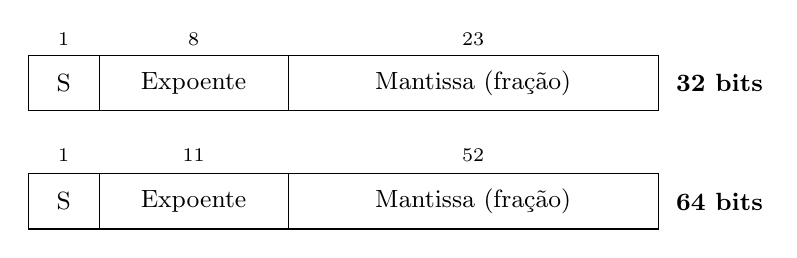
\begin{tikzpicture}[font=\small, every node/.style={inner sep=2pt}]
    % Formato simples: 1 + 8 + 23
    \draw (0,0) rectangle (0.9,0.7);   \node at (0.45,0.35) {S};
    \draw (0.9,0) rectangle (3.3,0.7); \node at (2.10,0.35) {Expoente};
    \draw (3.3,0) rectangle (8.0,0.7); \node at (5.65,0.35) {Mantissa (fração)};
    \node[above] at (0.45,0.75) {\scriptsize 1};
    \node[above] at (2.10,0.75) {\scriptsize 8};
    \node[above] at (5.65,0.75) {\scriptsize 23};
    \node[right] at (8.15,0.35) {\textbf{32 bits}};
    % Formato duplo: 1 + 11 + 52
    \draw (0,-1.5) rectangle (0.9,-0.8);   \node at (0.45,-1.15) {S};
    \draw (0.9,-1.5) rectangle (3.3,-0.8); \node at (2.10,-1.15) {Expoente};
    \draw (3.3,-1.5) rectangle (8.0,-0.8); \node at (5.65,-1.15) {Mantissa (fração)};
    \node[above] at (0.45,-0.72) {\scriptsize 1};
    \node[above] at (2.10,-0.72) {\scriptsize 11};
    \node[above] at (5.65,-0.72) {\scriptsize 52};
    \node[right] at (8.15,-1.15) {\textbf{64 bits}};
  \end{tikzpicture}
  \caption{Campos dos formatos simples (32 bits) e duplo (64 bits) da IEEE-754.}
  \label{fig:ieee754}
\end{figure}

Além do zero, o formato prevê valores especiais: infinito e \emph{NaN} (\emph{not a number}),
usado para resultados indefinidos como $0/0$. Dois eventos precisam ser previstos no programa:

\begin{itemize}
  \item \textbf{\emph{overflow}} --- o expoente é grande demais para caber no campo;
  \item \textbf{\emph{underflow}} --- o valor é tão pequeno (ou o expoente negativo tão grande) que
        não é representá vel.
\end{itemize}

Na prática, é por isso que a comparação de valores \texttt{REAL} exige tolerância: nunca se testa
``igual a zero'', mas ``menor que um valor mínimo''.

\begin{atencao}
Cálculos com \texttt{REAL} podem acumular erro e nunca fechar exatamente no valor esperado. Em
lógicas que dependem de comparação de reais --- nível, vazão, posição --- use sempre uma faixa de
tolerância definida no projeto, e registre essa escolha na documentação do programa.
\end{atencao}

\index{IEEE-754}\index{ponto flutuante}

\section{Dados estruturados, textos e arranjos}

Além dos tipos elementares existem dados que agrupam outras informações:

\paragraph{Tipos estruturados.} Várias variáveis de tipos possivelmente diferentes agrupadas em um
único nome. O exemplo mais presente na prática é o bloco de temporização: uma variável \texttt{TON}
disponibiliza internamente

\begin{itemize}
  \item \texttt{Timer\_01.PRE} --- valor de preset, que é do tipo \texttt{DINT};
  \item \texttt{Timer\_01.ACC} --- tempo acumulado, \texttt{DINT};
  \item \texttt{Timer\_01.EN} --- condição de funcionamento, \texttt{BOOL};
  \item \texttt{Timer\_01.DN} --- fim da contagem, \texttt{BOOL}.
\end{itemize}

Entender essa estrutura é o que permite, por exemplo, exibir o tempo acumulado na supervisão.

\paragraph{Tipos customizados.} Blocos de instrução definidos pelo usuário, com as variáveis
escolhidas por ele --- por exemplo, um bloco \texttt{VALVULA\_ON\_OFF} com os parâmetros
\texttt{LIGA}, \texttt{DESLIGA} e \texttt{STATUS}, todos \texttt{BOOL}.

\paragraph{Texto.} O tipo \emph{string} é uma sequência de caracteres. Em muitos controladores ocupa
85 bytes, com a estrutura da Tabela~\ref{tab:string}.

\begin{table}[H]
  \centering
  \caption{Organização típica de uma \emph{string} de 85 bytes.}
  \label{tab:string}
  \begin{tabular}{l l}
    \toprule
    Bytes & Conteúdo \\
    \midrule
    0--1 & \emph{offset} e comprimento máximo (0 a 80 bytes) \\
    2--3 & Comprimento atual \\
    4--83 & Caracteres que formam a palavra ou a frase \\
    84 & Terminador \\
    \bottomrule
  \end{tabular}
\end{table}

\paragraph{Arranjos.} Um \emph{array} armazena variáveis de mesmo tipo, em vetor ou matriz. Por
exemplo, \texttt{ARR\_INT[0..99] OF INT} cria 100 posições de inteiros; o acesso a cada posição é
feito pelo índice: \texttt{ARR\_INT[0]} é a primeira, \texttt{ARR\_INT[1]} a segunda, e assim por
diante.

\section{Arquitetura e mapa de memória do CLP}

As memórias de um controlador não têm todas a mesma função. A memória de \emph{programa} guarda um
conteúdo fixo, e a memória de \emph{dados} guarda o que varia durante a execução. Na prática, o mapa
de memória se divide em seis áreas:

\begin{figure}[H]
  \centering
  
\includegraphics[width=0.90\linewidth]{06-mapa-memoria.pdf}
  \caption{Áreas do mapa de memória de um controlador programável.}
  \label{fig:mapa-memoria}
\end{figure}

\begin{table}[H]
  \centering
  \caption{As seis áreas do mapa de memória do CLP.}
  \label{tab:areas-memoria}
  \begin{tabular}{p{3.2cm} p{2.2cm} p{8.6cm}}
    \toprule
    Área & Tecnologia & O que guarda e quem acessa \\
    \midrule
    Executiva
      & ROM ou EPROM
      & Sistema operacional (\emph{firmware}) que gerencia o hardware; somente leitura para o
usuário \\
    Do sistema
      & RAM
      & Resultados e operações intermediárias do próprio sistema; é um rascunho, não acessível ao
usuário \\
    Imagem de E/S
      & RAM
      & Status das entradas (gravado após a leitura) e status das saídas (gravado após o
processamento) \\
    De dados
      & RAM
      & Valores de temporização, contagem, aritmética, PID e manipulação de dados \\
    Do usuário
      & RAM ou RAM/EEPROM/Flash
      & O programa do usuário, lido pela CPU instrução por instrução \\
    Retentiva
      & RAM com bateria ou área dedicada
      & Preserva o valor após o desligamento; a variável precisa ser declarada como retentiva \\
    \bottomrule
  \end{tabular}
\end{table}

A \textbf{memória retentiva} merece atenção: em alguns controladores existe uma área exclusiva, e a
marca de retenção é feita na declaração da variável; em outros, não há divisão e toda a RAM é
mantida por bateria. O sintoma de bateria fraca é o comportamento que ``muda sozinho'' após uma
falta de energia --- assunto do Capítulo~\ref{cap:manutencao}.

\begin{pratica}
Em um controlador com programador disponível, crie quatro variáveis: um \texttt{BOOL}, um
\texttt{INT} no limite superior ($32.767$), um \texttt{DINT} e uma \texttt{STRING}. Depois:
(a) some 1 ao \texttt{INT} de valor máximo e observe o que acontece;
(b) inverta um número negativo para positivo e escreva o resultado;
(c) veja no \emph{software} de programação em que área de memória cada variável foi alocada.
O resultado da letra (a) é uma das causas mais frequentes de defeito intermitente em programas reais.
\end{pratica}

\begin{exercicios}
\begin{enumerate}[label=\alph*)]
  \item Classifique uma memória \emph{flash} pelos quatro critérios da
        Tabela~\ref{tab:classificacao-memoria}.
  \item Quantos bits de endereçamento exige uma memória de $65.536$ bits com palavras de 8 bits?
  \item Explique, sem usar fórmula, por que o \texttt{UINT} vai de 0 a 65.535 e o \texttt{INT} de
        $-32.768$ a $32.767$.
  \item Represente $-5$ em complemento de dois com 8 bits, mostrando os dois passos.
  \item No formato simples da IEEE-754, quantos dígitos significativos se pode esperar de um
        \texttt{REAL}? E no duplo? Relacione com a largura da mantissa
        (Figura~\ref{fig:ieee754}).
  \item Por que uma comparação de igualdade entre duas variáveis \texttt{REAL} é uma má prática?
  \item Explique o princípio da forte tipação adotado pela norma IEC 61131-3. Por que a linha
        \texttt{rVazao := rVazao + iAjuste;} (sendo \texttt{rVazao} do tipo \texttt{REAL} e
        \texttt{iAjuste} do tipo \texttt{INT}) causa erro de compilação, e como ela deve ser
        escrita para ser executada pelo CLP?
  \item Um programa usa \texttt{Timer\_01.ACC} para calcular a taxa de produção. Em qual área do
        mapa de memória (Tabela~\ref{tab:areas-memoria}) esse valor está armazenado?
  \item Um técnico relata que a contagem de peças do turno anterior se perdeu depois de uma falta de
        energia. Em que área de memória a variável provavelmente estava alocada, e como corrigir o
        programa?
\end{enumerate}
\end{exercicios}
